\chapter{A Query Obfuscation Game}
The goal of this thesis is to research how well humans obfuscate private search queries. Therefore, we need appropriate, data about sensitive queries and possible corresponding obfuscations. Since the collection of the necessary data is a quite monotonous task, we decided to develop a web game. Using gamification makes this task more fun and potentially increases user participation. In this chapter, we give an overview of our game, its game design elements, and the development process.

\section{Game Overview}
\label{overview}
Our game, City of Rebellion, is a version of Page Hunt but with a significant difference. Just like in Page Hunt, players are shown a web page that they have to retrieve by submitting a query to a search engine. But instead of finding a search query for the web page, the associated query is already provided (see (2) in Fig~\ref{fig:game_interface}). The task of the players is to hide the sensitive information need as well as possible by obfuscating the given query while still retrieving the target document.
For the obfuscation, users are allowed to use any words or phrases, except the ones that make up the original query. Queries that contain one or more forbidden words are not accepted and the player will get an error message.
To help users to fulfill the task, a list of 10 keywords is presented (see (3) in Fig \ref{fig:game_interface}). Players will receive points if the query they submitted retrieves the target document.\par
\begin{figure}[h]
    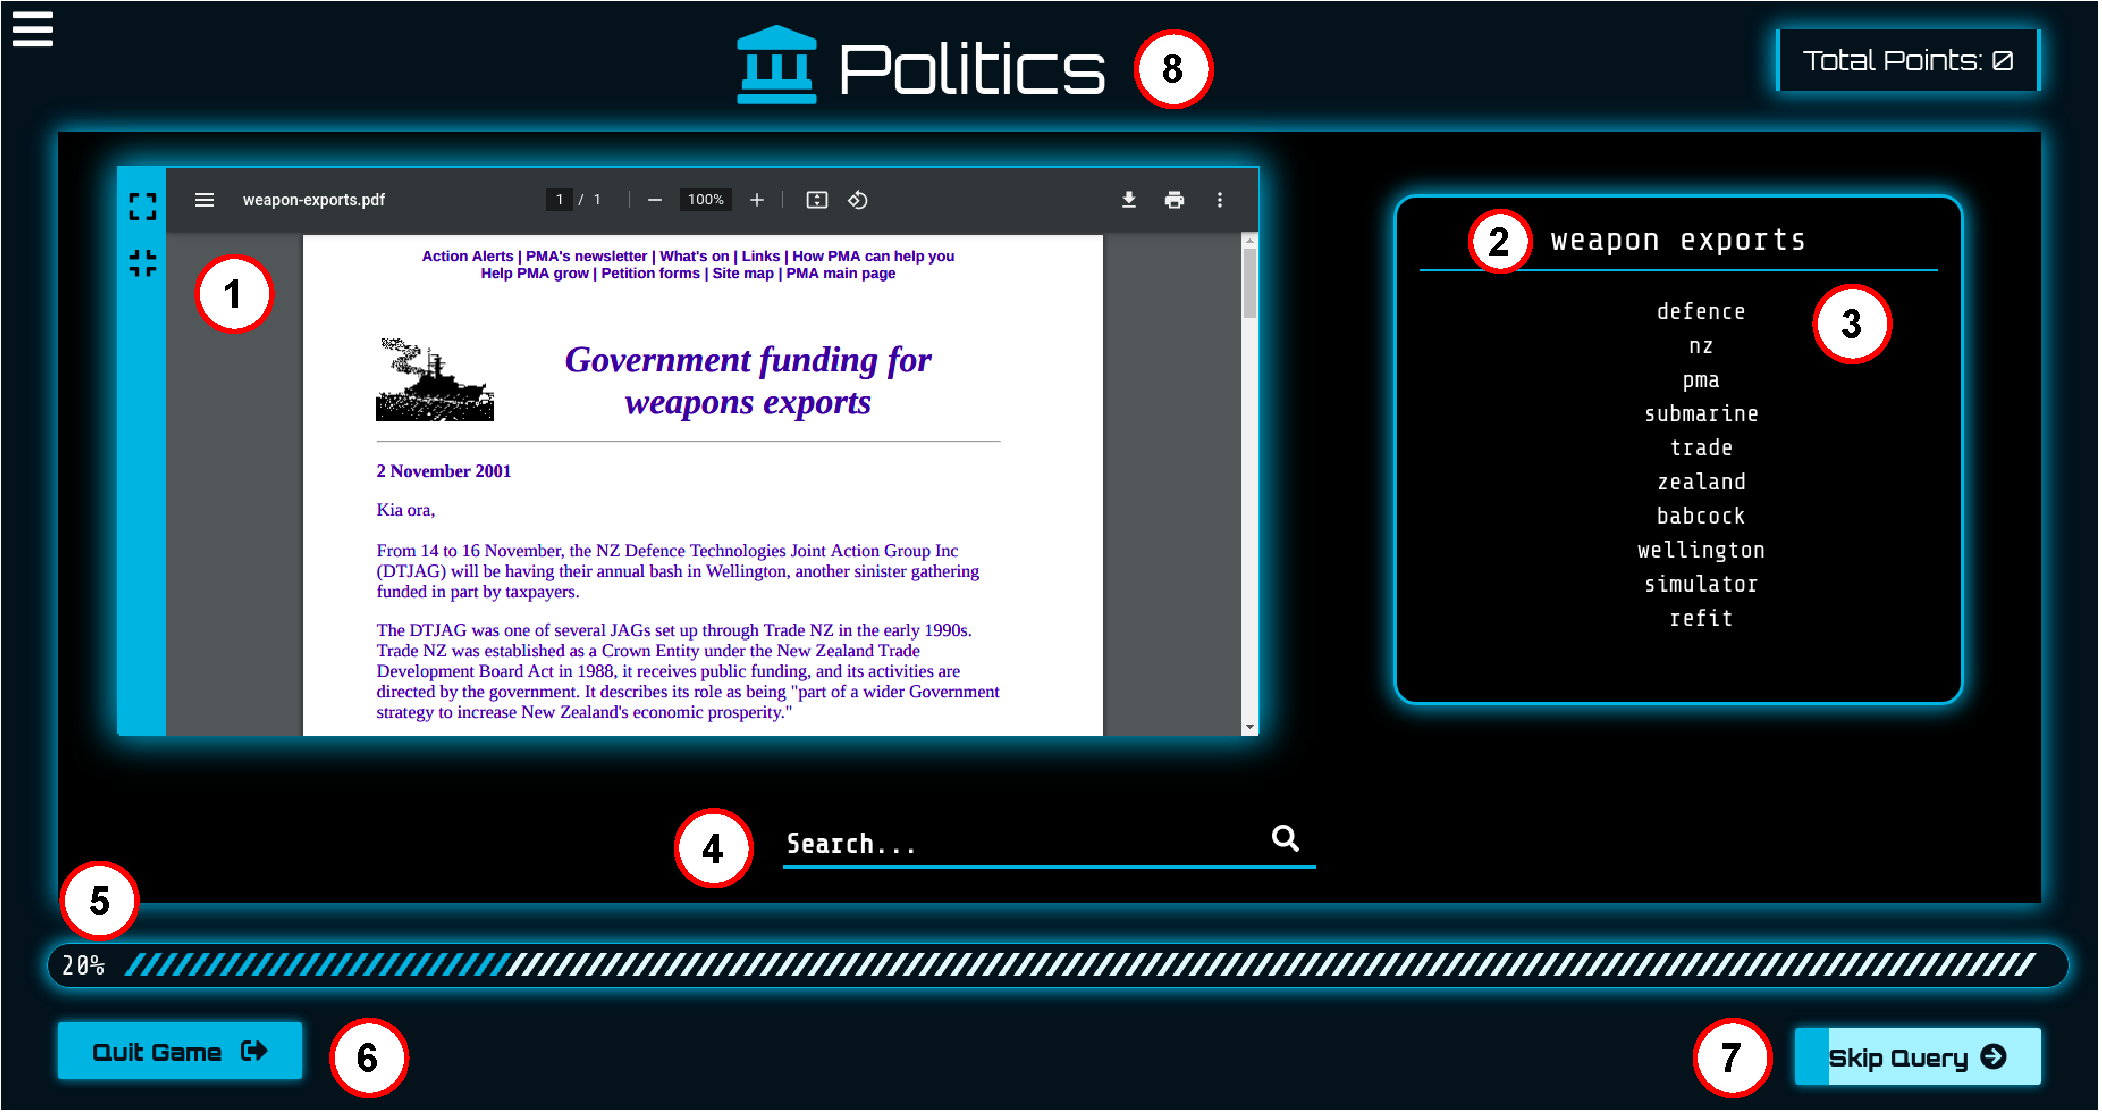
\includegraphics[width=1.0\textwidth]{graphics/game/game_description_all_elements.pdf}
    \caption{A screenshot of the main game interface, containing (1) the target document, (2) the associated query, (3) a list of auxiliary keywords, (4) a search field to enter queries, (5) a progress bar, (6, 7) buttons to skip a query or quit the game and (8) a header to show the selected category.}
    \label{fig:game_interface}
\end{figure}
In order to be able to go into more detail about the individual game elements, later on, we will briefly explain a typical game course in the following.\par
If users are playing for the first time, they get an introduction that describes the fictional scenario in which they find themselves. In this context, it is also explained what their task is and how they can solve it. Afterward, players get redirected back to the home screen, the starting point of the game. This home screen consists of a city map with different districts, each representing a different category (see Figure~\ref{fig:city}). Players may now start a new game by selecting a category and then clicking on the corresponding district on the map. The game interface will then open and participants can think of a suitable obfuscated query. If they submit an appropriate query, they get points and may continue the game or try to achieve more points.\\
In total, a game lasts five rounds. Once these are completed, players automatically are returned to the home screen. 
\begin{figure}[h]
    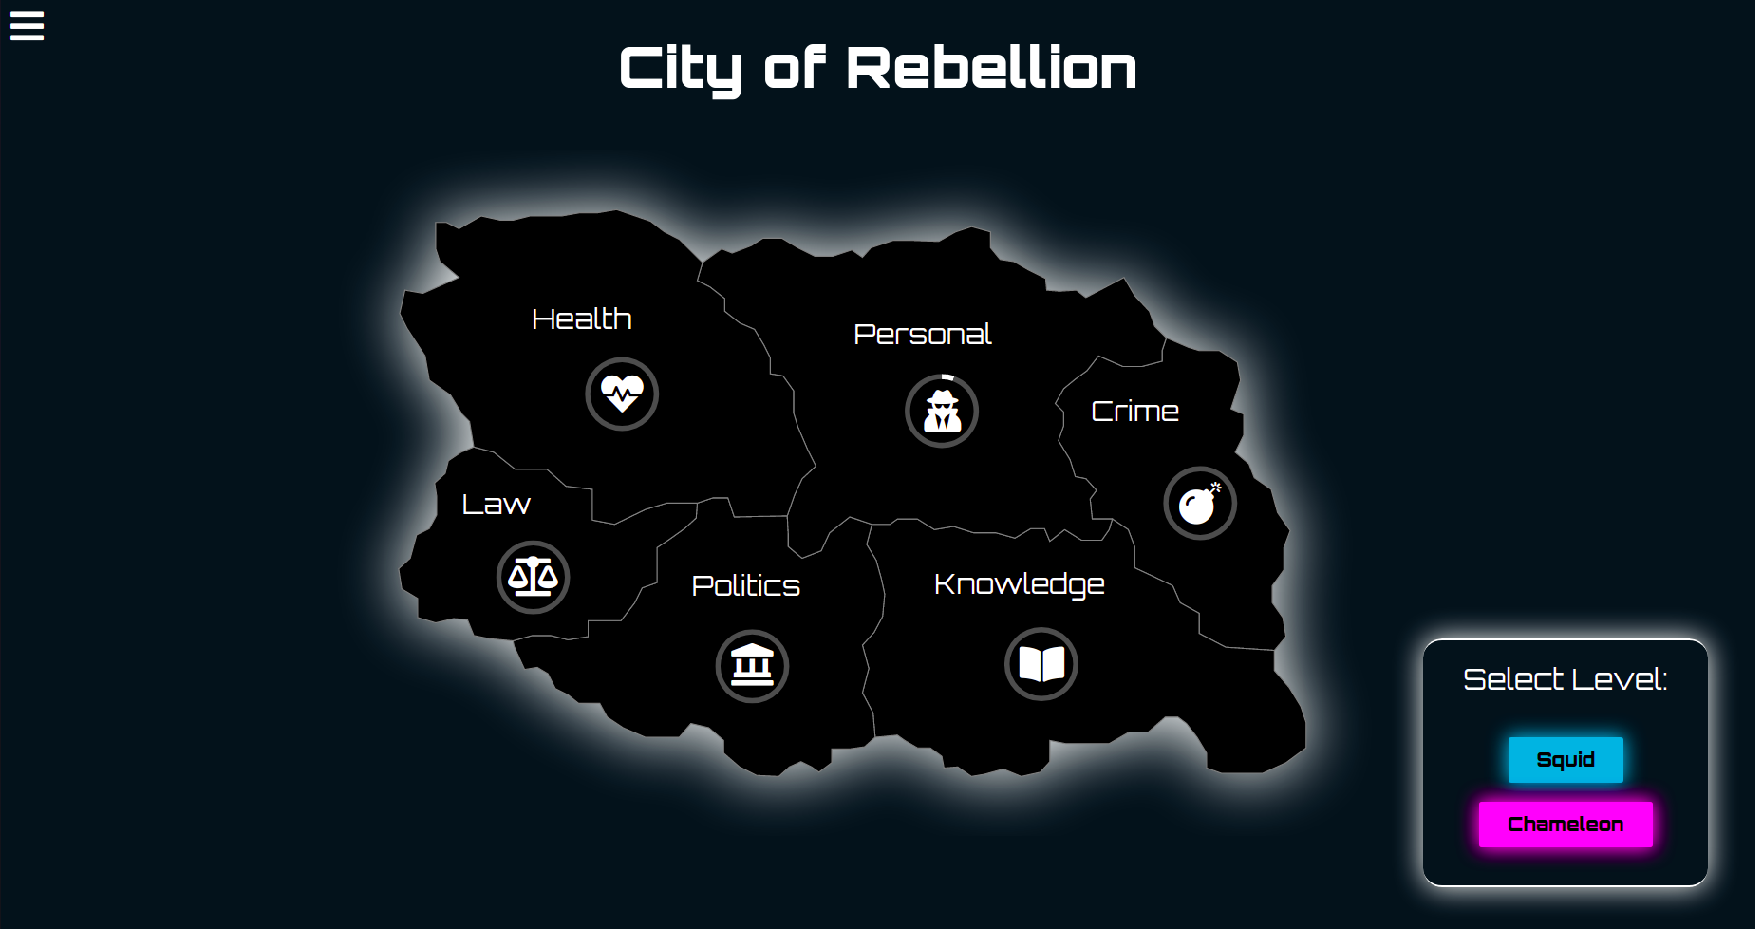
\includegraphics[width=1.0\textwidth]{graphics/game/city_levels.pdf}
    \caption{A screenshot of the game's home screen where players can click on a district of the city map to start a new game in the selected category.}
    \label{fig:city}
\end{figure}

\section{Game Properties}
\subsection*{Narrative}
To create a more meaningful experience, we thought of a background story for the game. The setting is a dystopia in which the government passed a law that completely abolishes data protection, turning the nation into a police state. The player takes on the role of a rebel in a resistance group. This group is helping others to hide their private information need by obfuscating queries before submitting them to a search engine.
This story is presented to users as a part of the game instructions and introduction (see Figure~\ref{fig:intro}).
\begin{figure}[h]
\centering
    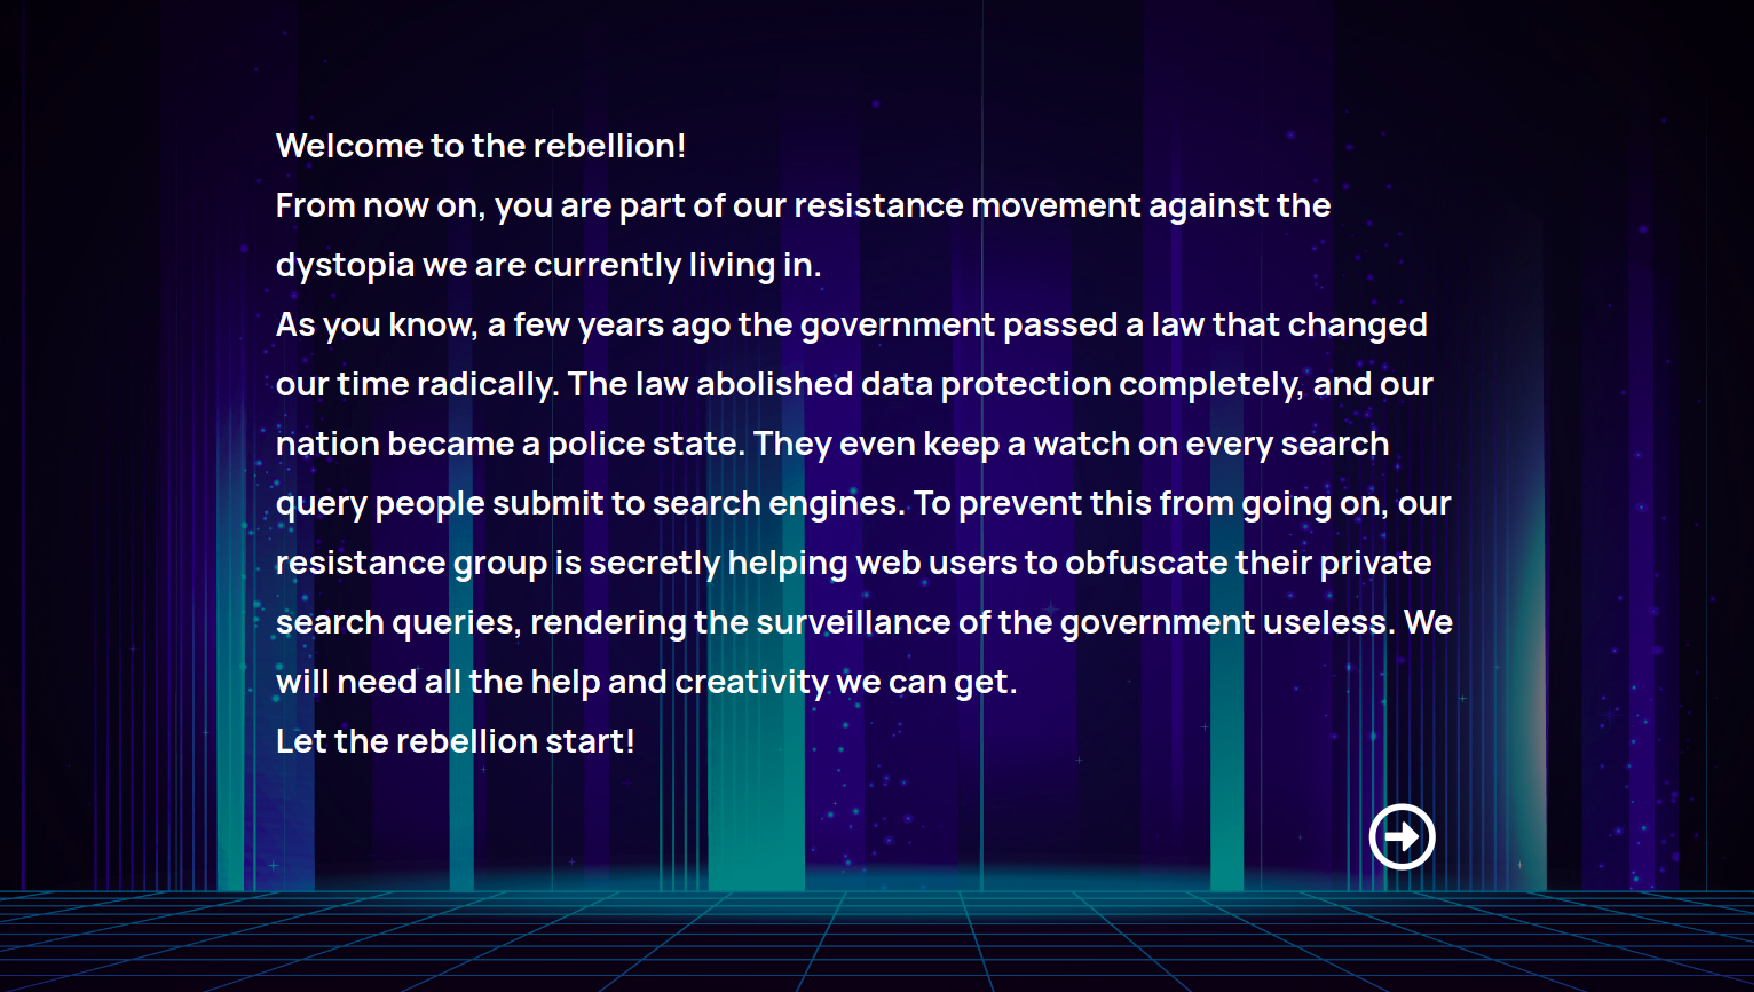
\includegraphics[width=1.0\textwidth]{graphics/game/introduction (1).pdf}
    \caption{A screenshot of the introduction that explains the background story of the game and the role of the player.}
    \label{fig:intro}
\end{figure}
This scenario is also reflected in the game design and structure. 
First of all, the starting point of the game is designed as a city map, which is supposed to represent the player's hometown and also serves as a starting point for a new game round (see Figure~\ref{fig:city}). The city makes things a bit more personal and at the same time offers a clear design for the categories which is in line with the story. In addition, the overall game design is futuristic to make the concept of a future dystopia more realistic.\par
With the help of an interesting scenario, we want to increase participation and the performance of players. For this reason, we have developed a background story that addresses the problem of search privacy and is linked to a widely known dystopian scenario. The emergence of a surveillance state, that collects profiles of all web users through their search queries, appears in many video games, books, and movies.
With this, we want to bring the motivation of this thesis closer to the users as well as create a recognition value and give players the possibility to immerse deeper into the scenario.

\subsection*{Levels}
Our game has two levels, Squid and Chameleon. The name givers of the levels are both animals that are masters of camouflage and thus reflect the task of players to obfuscate sensitive information needs. In the beginning, only the first level Squid can be played. When a player has successfully obfuscated five queries, a second level Chameleon gets unlocked (see Figure~\ref{fig:city}). The second level is more or less identical to the first, except for two small differences. First, the color scheme of the second level is purple in contrast to the blue Squid level. The second and critical difference is that now players will lose points if they use any auxiliary keywords. With this technique, we want to make sure that players have to become more creative in their obfuscation attempts. We also want to provide more variety to the game. Furthermore, adding levels to the game suggests progress to the players, creating a sense of acknowledgment.

\subsection*{Points}
Players receive points for successfully retrieving the target document while obfuscating the original query. The points are divided into different categories and are loosely based on some evaluation measures for information retrieval systems.
\begin{figure}[h]
\centering
    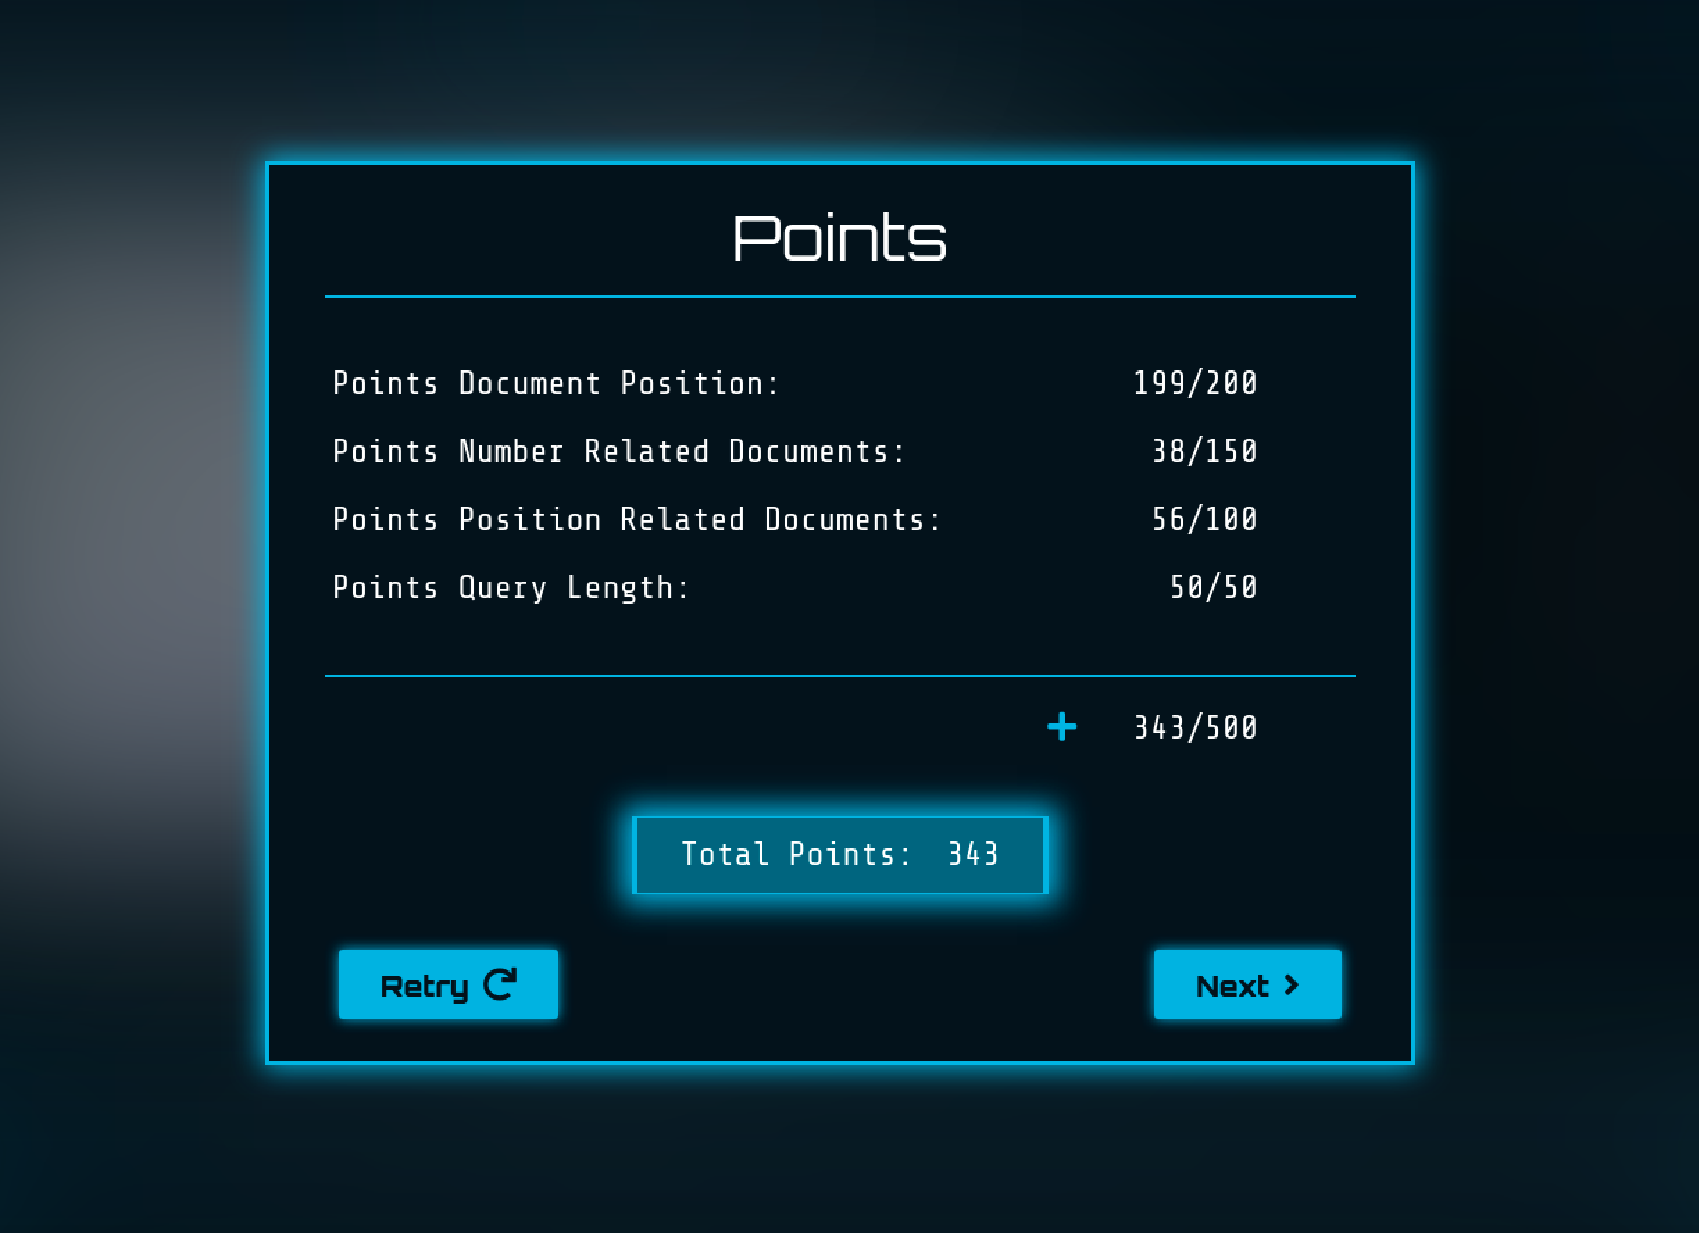
\includegraphics[width=0.8\textwidth]{graphics/game/points_cropped.pdf}
    \caption{A screenshot of the score board that opens up if a player retrieved the target document.}
    \label{fig:points}
\end{figure}
First of all, let's look at the points calculation of the first level Squid.
\newpage
\noindent Four factors play a role here:
\begin{enumerate}
    \item The position of the target web page inside the search response,
    \item the number of related documents that would also be retrieved if the original query were to be submitted,
    \item the average position of these related documents inside the response, and
    \item the length of the obfuscated query.
\end{enumerate}
Players could receive a maximum total of 500 points per round. First of all, it is checked whether the target document is among the top 8000 positions, which the search engine returns as soon as the player submitted his search query. If this is not the case, the player receive an error message and has to revise and resubmit his search query. If, however, the document was found by the search engine, the number of relevant documents, their average positioning, and the length of the player's search query are calculated. These variables are then used to calculate the corresponding points.\par
\begin{table}[t]
\centering
    \caption{(a) Steps of the algorithm to compute points for the position of the target web page. (b) Example of the points calculation for the average position of found related documents.}
    \label{tab:docpos}
\subfloat[Subtable 2 list of tables text][Target document]{
\begin{tabular}[t]{cc}
\toprule
Position & Points\\
\midrule
1 - 10&200\\    
11 - 20&199\\    
21 - 30&198\\ 
$\cdots$ & $\cdots$\\ 
101 - 120&190\\ 
121 - 140&189\\ 
$\cdots$ & $\cdots$\\ 
2001 - 2050&95\\ 
2051 - 2100&94\\ 
$\cdots$ & $\cdots$\\ 
5001 - 5100&35\\ 
5101 - 5200&34\\ 
$\cdots$ & $\cdots$\\ 
> 7000 & 10\\
\bottomrule
\end{tabular}}
\qquad
\subfloat[Subtable 3 list of tables text][Related web pages]{
\begin{tabular}[t]{cc}
\toprule
Average Position & Points\\
\midrule
x < 160 & 100 \\  
$161 < x \leq 320$  & 98\\ 
$320< x \leq 480$ & 96 \\ 
$\cdots$ & $\cdots$\\
\bottomrule
\end{tabular}}
\end{table}
For the web page's position (1.) a maximum of 200 points is possible. The further down the web page is positioned, the fewer points the player receives. To compute the final points, we divide the 8000 possible positions, on which the web page could be placed into steps, and, based on these steps, deduct points from the 200 starting points. In the range of the positions \mbox{1-100}, one point is deducted for every 10 steps down in the positioning, from \mbox{101-2000} it is 20 steps, from \mbox{2001-5000} 50 steps, from \mbox{5001-7000} 100 steps and from a positioning of 7001 and above players constantly receives 10 points as a minimum (see Table~\ref{tab:docpos}~(a)).\par
For the number of related documents (2.) players may reach 150 points at max. For this purpose, the number of relevant documents found is simply converted directly into points, for example, 24 found documents result in 24 points. Since we saved the IDs of 300 related documents for each query, players may retrieve more than 150. In this case, they simply get the maximum of points (see Table~\ref{tab:docpos}~(b)).\par
The third factor (average position of related documents) brings a maximum of 100 points. The computation is similar to the calculation of the points that players can achieve for the positioning of the target web page. For this purpose, the 8000 positions that the search engine returns as a maximum are divided into levels of 160 positions each. For each level down, which means a worse positioning, two points are deducted from the initial 100 (see Table~\ref{tab:docpos} (b)). For example, if the average position is $\leq$ 160, players receive 100 points, if it is between 161 and 320, 98 points are awarded, and so on.\par
And finally, players get points for the query length. The maximal number of points users can achieve here is 50. Players receive the maximum number of points if their query is shorter or the same length as the original query. For each additional word, one point is deducted. In this context, length is defined as the number of words the query consists of.\par
In the second level Chameleon, the same aspects play a role in calculating the points. This means that players receive points for the same criteria as before. In addition, however, the use of the suggested keywords has a negative effect on the achievable points. When players use one or more of the provided keywords, they lose points. This works as follows: Each keyword has a certain value, which is reflected by its position in the list. The value decreases with each word in descending order. Thus, the first word is worth 100 points, the second 90, and so on. When a player submits a query, the values of the keywords used for it are summed up and then subtracted from the total number of points. This means that players can lose up to 550 points which would result in a negative score. We implemented this kind of point calculation to encourage the players to give more thought to the formulation of their search queries. 

\subsection*{Performance Graphs}
In contrast to the competitive leaderboards, performance graphs show the individual performance of players. This can create a sense of mastery for the participants, motivating them to invest more time in the game \cite{wirkungGamificationBuch}. We implemented two kinds of graphs. One kind shows the performance of users (collected points and number of successfully obfuscated queries) over time (see Figure~\ref{fig:statistics}. The second kind shows how many queries have already been solved in each category.
\begin{figure}[h]
    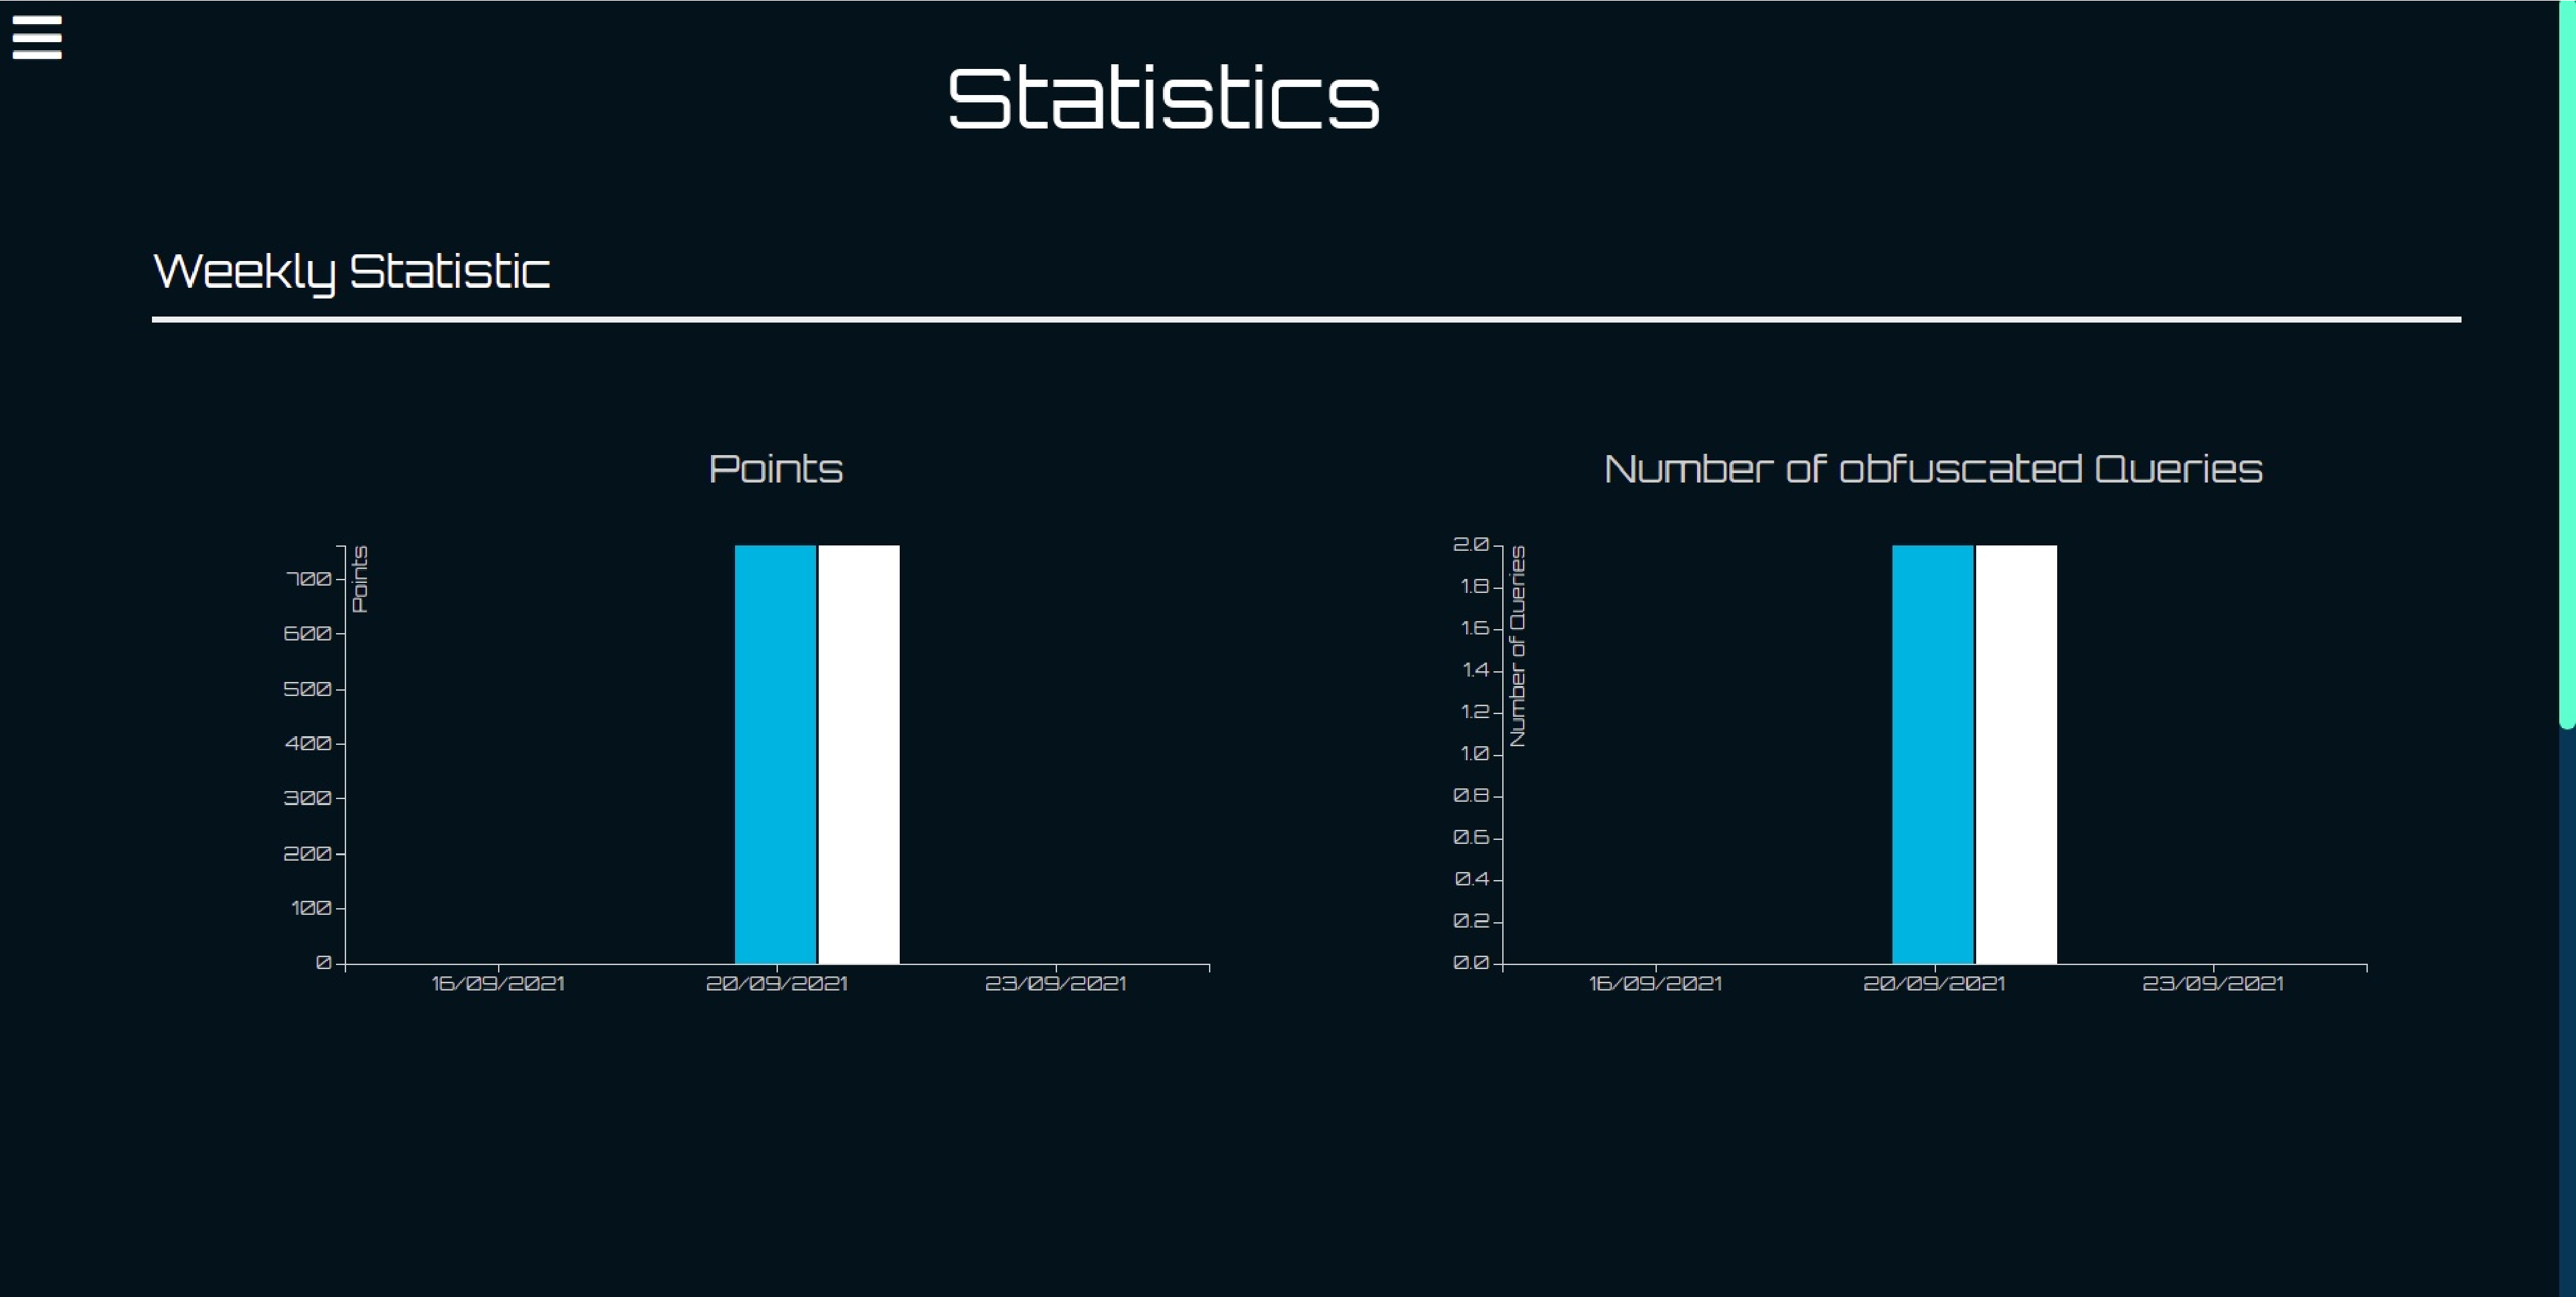
\includegraphics[width=1.0\textwidth]{graphics/game/statistics.pdf}
    \caption{A screenshot of a user's performance graphs. One graph (left) shows how many points a player received for each level and in total for every day he or she played. The other graph (right) shows how many queries the player successfully obfuscated over time.}
    \label{fig:statistics}
\end{figure}

\subsection*{Usernames}
When a participant visits the web page of the game for the first time, a new entry in our MongoDB database is created with a random user name. This username consists of an adjective followed by a surname. It is used to identify a player inside the leaderboards and can be changed to fit the player's preferences (see Figure~\ref{fig:username}). The username is a game design element that creates more freedom for players as well as customization.
\begin{figure}[h]
    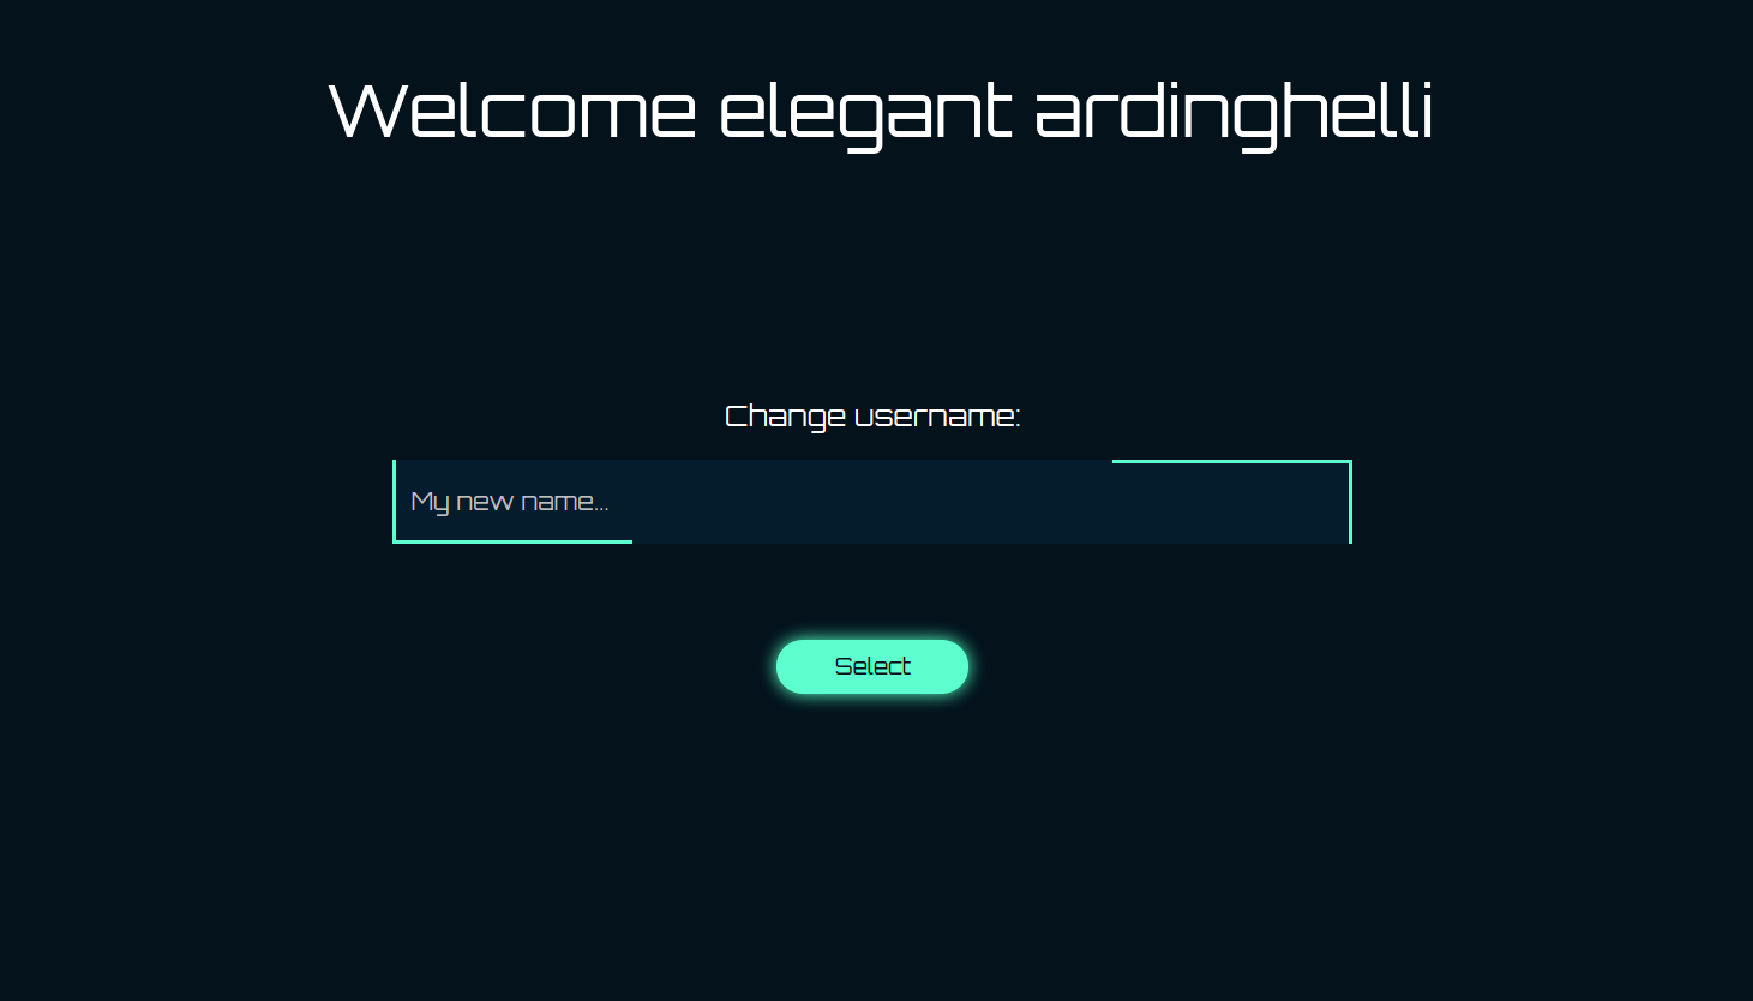
\includegraphics[width=1.0\textwidth]{graphics/game/username (1).pdf}
    \caption{A screenshot of the form which allows players to choose their own usernames.}
    \label{fig:username}
\end{figure}

\subsection*{Leaderboards}
We have designed three leaderboards, one for each level and a third one that combines the points from both levels to an overall performance (see Figure~\ref{fig:leader}). With this, we want to achieve a sense of challenge between the users and motivate them to climb to the top by playing more and/or better than the others. We designed three leaderboards to prevent the demotivating effect one could have. Now, players have a greater chance to be at the top of at least one of the boards. Furthermore, participants can gain a lot of points in a short period which makes it easier to raise inside this hierarchy. We added this game design element to help us to increase the user performance, thus, collecting more data.
\begin{figure}[h]
    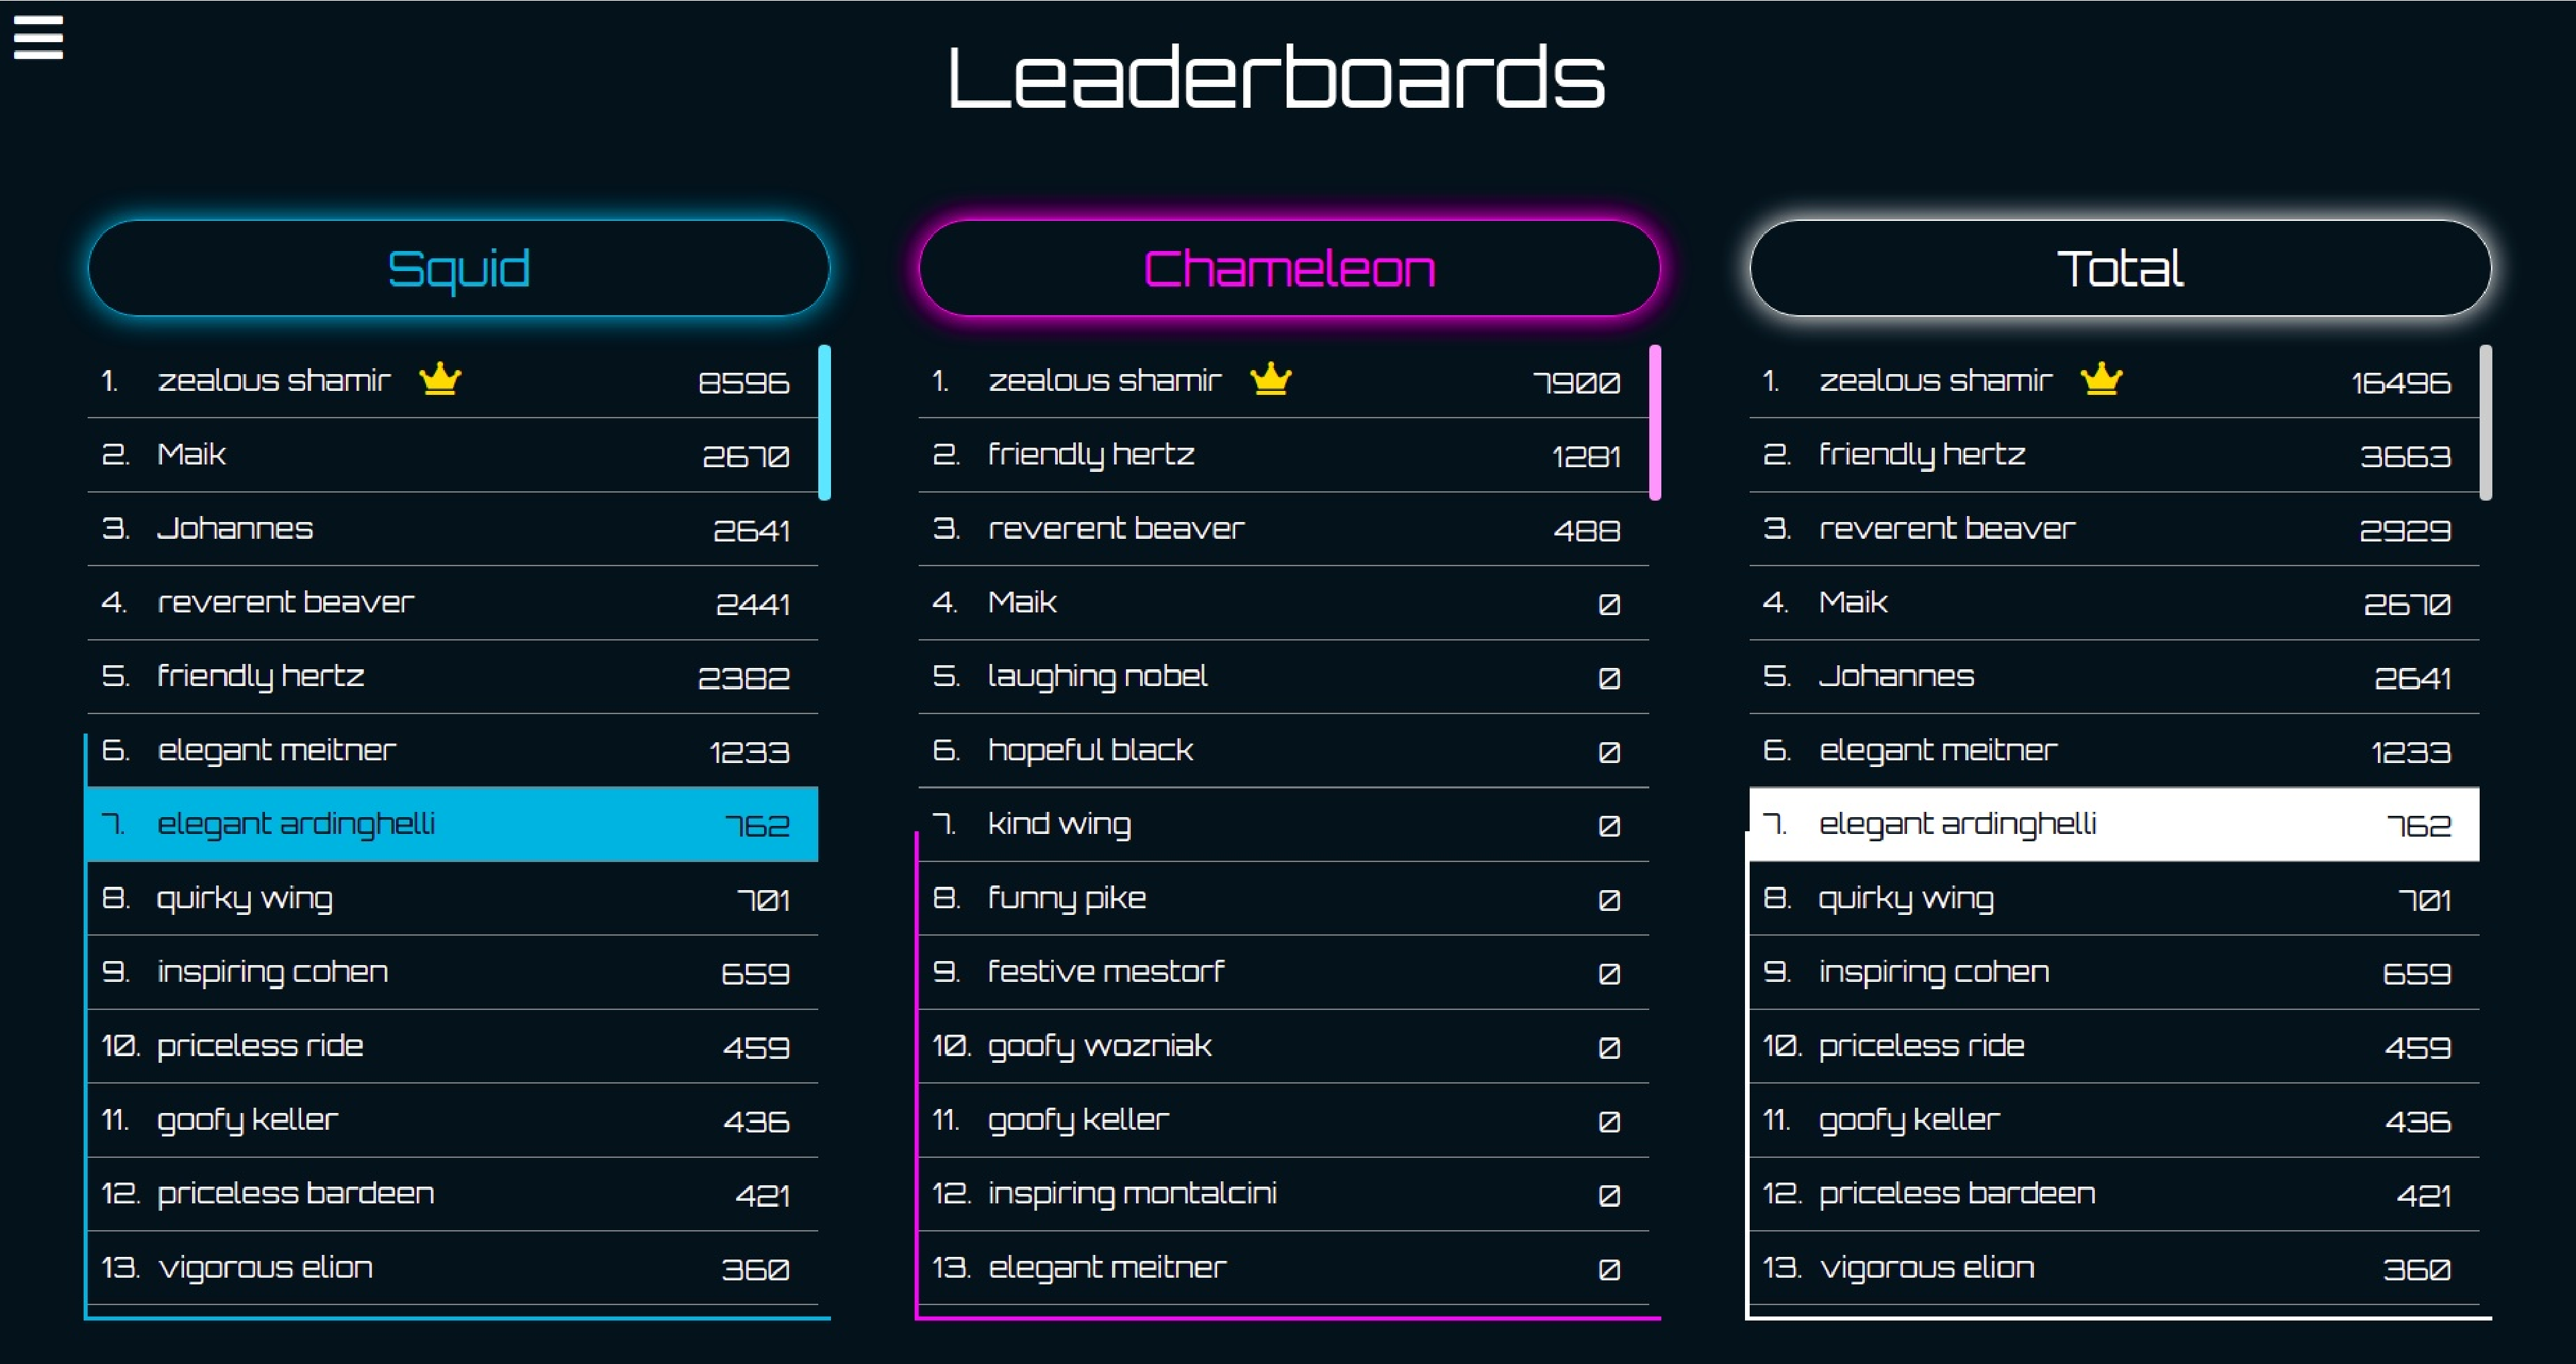
\includegraphics[width=1.0\textwidth]{graphics/game/leaderboards.pdf}
    \caption{A screenshot of the three different leaderboards, one for each level and one for an overall performance.}
    \label{fig:leader}
\end{figure}

\subsection*{Categories}
To make things more interesting and to create more freedom of choice, players may choose between six categories of query types. These categories correspond to specific subject areas into which the queries could be classified, namely Health, Personal, Crime, Knowledge, Law, and Politics (see Figure~\ref{fig:city} and Table~\ref{tab:category}). This potentially has a positive effect since players may choose to play game rounds in a category they are either interested in or have further knowledge about~\cite{gamifiedSearch}. This offer makes the game more interesting and diverse since it creates meaningful choices and demonstrates preferences. It is a game technique that addresses the feeling of empowerment and the creativity of players~\cite{actionableGamification}, thus, satisfying psychological needs.

\subsection*{Progress Bar}
We implemented two different kinds of progress bars in the game.
One kind of progress bar is part of the main game interface and indicates in which game round a player currently is (see Figure~\ref{fig:game_interface}). It acts as a simple feedback function that reflects the player's status. Furthermore, it serves as a goal and motivates people to finish the game round by addressing the psychological need to finish incomplete things \cite{actionableGamification}. The other progress bar is part of the home screen included in the city map. On this map, a donut chart is drawn for each category, showing how many queries from that category have been successfully obfuscated (see Figure~\ref{fig:category1}, \ref{fig:category2}) in the selected level.
\begin{figure}[ht!]
    \begin{minipage}[b][][b]{0.46\textwidth}
    \centering
    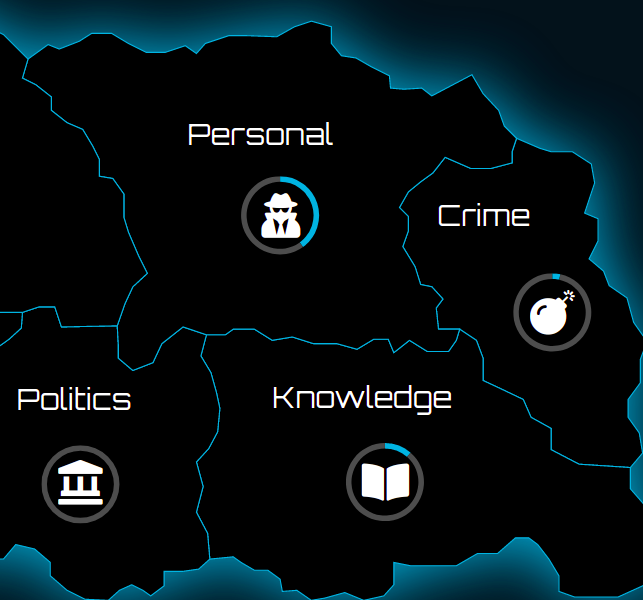
\includegraphics[width=0.9\textwidth]{graphics/game/city_category.png}
    \caption{A screenshot of the category graphs in the level Squid.}
    \label{fig:category1}
    \end{minipage}
    \hfill
    \begin{minipage}[b][][b]{0.46\textwidth}
    \centering
    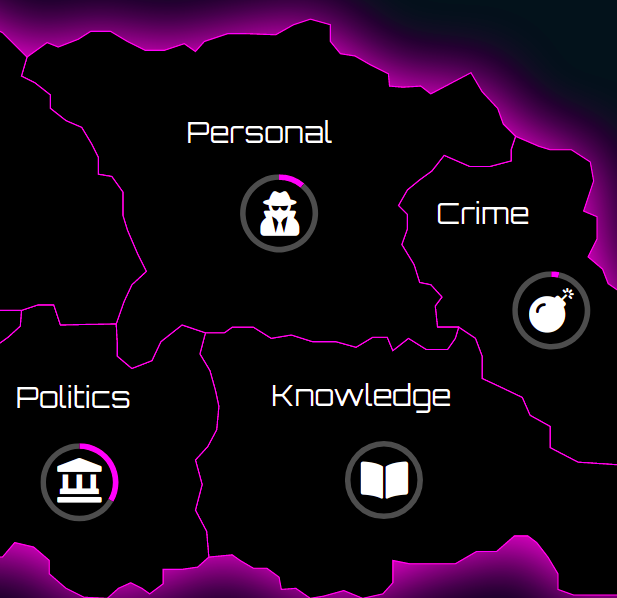
\includegraphics[width=0.87\textwidth]{graphics/game/city_category_2.png}
    \caption{A screenshot of the category graphs in the level Chameleon.}
    \label{fig:category2}
    \end{minipage}
\end{figure}

\subsection*{Other Features}
We implemented a few more features that are not directly typical game design elements but also help to make the user experience more pleasant. To prevent frustration and make the navigation inside the game easier, we added two buttons in the main game interface. These buttons allow the players to either quit the game and return to the home screen or to skip a query after 60 seconds if they get stuck (see 6. and 7. in Figure~\ref{fig:game_interface}). Another feature is the Retry button. Every time, players successfully obfuscated a query they get the possibility to continue with the next query or try to improve their current score. The idea behind this button is to give players the chance to improve their performance. The auxiliary keywords were taken from the list of keywords that the search engine ChatNoir~\cite{chatnoir} extracted for the corresponding web page.

\section{Game Development}
In this section, we explain the different components of the game development by describing the process of collecting queries to obfuscate and rendering the target documents visually appealing. Afterward, we describe how and what data we collected for the evaluation.

\subsection{Sensitive Queries}
The first step we had to take was to create a collection of sensitive search queries. For this purpose, we consulted the AOL query logs, a collection of TREC Web track queries~\cite{anserini}, and a paper of Arampatzis et al.~\cite{arampatzis} from which we extracted suitable sensitive queries. The basis of our collection is a list of sensitive queries that Arampatzis et al. created \footnote{\url{http://lethe.nonrelevant.net/datasets/95-seed-queries-v1.0.txt}}. However, we skipped all queries with sexual or inappropriate content like \texttt{free porn movies}. These kinds of queries are certainly sensitive and should stay private but their content is unsuitable for our game, especially since we display relevant web pages. Skipping these unsuitable queries, allowed us to gather 82 queries for our collection out of the original 95. Furthermore, we extracted queries from a collection of sensitive TREC Web Track queries. These queries were particularly helpful for our evaluation since there exist annotated data on the information needs and relevant web pages. With this additional data, we are able to make even more well-founded statements about the obfuscation skills of players. The biggest sources for our collection are the AOL query logs, a huge collection of queries from various users. Here, we also ignored the pornographic and hateful contents. Additionally, inspired by these resources, we added some self-devised queries to our collection.
Overall, we assembled a list of 700 sensitive search queries. To group the queries into districts on the city map, we had to find suitable categories for the queries. Inspired by Arampatzis' paper \cite{arampatzis} and our list, we were able to derive six different categories in which we organized the queries (see Table~\ref{tab:category}).

\newpage
\begin{table}
\centering
\caption{The six different categories in which we organized the queries and the number of queries for each category.}
\label{tab:category}
\begin{tabular}[th]{ccc}
\toprule
Category & Example Query & Number of Queries\\
\midrule
Health & \texttt{folk remedies sore throat} & 65\\    
Personal & \texttt{cheating husbands} & 45\\    
Knowledge & \texttt{evidence for evolution} & 35\\ 
Crime & \texttt{forged passports} & 30\\ 
Law & \texttt{pregnancy discrimination laws} & 15\\ 
Politics & \texttt{weapon exports} & 15\\ 
\bottomrule
\end{tabular}
\end{table}

\subsection{Visual Enriching of Sensitive Documents}
\label{enriching}
To support users in obfuscating queries, we show them a relevant ClueWeb document for the sensitive query. For this task, we used the Elasticsearch-based search engine ChatNoir, a search interface for the two ClueWeb corpora and the Common Crawl~\cite{chatnoir}. It was developed especially for research purposes and has a freely accessible API~\cite{chatnoir}, allowing us to easily access the ClueWeb12 from which we chose the target documents for the sensitive queries. We decided to use the ClueWeb12 since web pages from 2012 often look better than those from 2009. This improves the graphic aesthetics of our game. Moreover, modern-looking web pages are more compliant with our futuristic background story. ChatNoir also provides additional data for each web document, such as a list of keywords, which we have adopted for the game (see Section \nameref{overview}). However, documents in the ClueWeb are not intended to be shown to humans because additional resources like CSS stylesheets or images are not included in the crawl. This means that most web pages are not well-formatted and are rather unsightly and chaotic. That would be disadvantageous for our game because you can not draw information from these documents easily. To counteract this issue, we have developed a strategy that allows us to make web pages visually pleasing again with the help of the web archive Wayback Machine. This works as follows (see Algorithm~\ref{alg:resources}):\par
First, we send a request to ChatNoir that returns the corresponding top three web documents. For each document, we extract the original URI and the time at which it was crawled. With these two pieces of information, we send a request to the Wayback Machine API. The response then tells us whether the web page exists inside the web archive or not. If the web page is not inside the archive, the algorithm repeats the process described above with the next document. Otherwise, we take the URL of the web page inside the Wayback Machine. Since there can exist several snapshots of the same web page inside the web archive, we save the URL of the version that was crawled in close temporal proximity to the wanted ChatNoir document. Next, we replace the links to the stylesheets and images in the ChatNoir document so that they point to the resources stored by the Wayback Machine. Therefore, we first extract all stylesheet links from the web page inside the Wayback Machine. This is done with the Python library Beautiful Soup and the URL we got from the web archive in the previous step. Next, we extract the stylesheet links from the ChatNoir web page and delete the part of the links that define the communication protocol. Afterward, we check for all stylesheet links of the ChatNoir web document if they are part of a web archive link. If this is the case, then the link inside the ChatNoir web page gets replaced by the link of the Wayback Machine. Afterward, the same is done for the image resources. In the last step, the changed ChatNoir web page is saved as a new HTML file.\\
We also deleted all links of the \texttt{<a>} tags from the file to prevent users from being redirected when they accidentally click on one of them.
\begin{algorithm}[t!]
	\caption{Change Resources}\label{alg:resources}
	\hspace*{\algorithmicindent} \textbf{Input:} Set Q of sensitive search queries \\
    \hspace*{\algorithmicindent} \textbf{Output:} HTML files with changed resources for queries in Q
	\begin{algorithmic}[1]
		\For {q in Q}
		    \State chatnoir\_response = request\_top\_3\_documents(q)
		    \For {document in chatnoir\_response}
		        \State archived\_document = closest\_snapshot\_in\_archive(document.uri, 
		        \State \hspace{9.7em} document.timestamp)
		        \If {archived\_document is not None}
                    \State replace\_stylesheets(document, archived\_document)
		          %\State{\# does the same exchange of links for the images}
		          \State replace\_images(document, archived\_document) 
		          \State render\_enriched\_document(document)
		          \State save(document)
		        \EndIf
		  \EndFor
	    \EndFor
	\end{algorithmic} 
\end{algorithm}

\newpage
\subsection{Selection of Queries}
Finally, we had to decide which queries should become part of our game. For the selection process three criteria were taken into consideration:
\begin{enumerate}
    \item The target document is part of the web archive.
    \item The resources of the target document could be enriched enough to be visually pleasing.
    \item The target document is relevant for the sensitive query.
\end{enumerate}
First of all, if neither of the top three documents of a query was found inside the web archive, then the query was considered to be unsuited. That is because the look of a web page is important for the game (see Section \nameref{enriching}). Next, we had a look at all queries for which at least one of the top web pages could be visually enriched. Not all web pages could be restored by our algorithm and were therefore unsuited to be part of the game. The last criterion for a query or rather a web page was if it contains relevant and helpful data that could support the players in their obfuscation attempts. Only if at least one of the web pages for a query met all these criteria, the query was included in our game. This selection process was very strict and only 50\% of the regarded queries passed it. After the completion of this process, the selected documents were converted and saved as PDFs. The reason for this conversion was the fact that the web pages needed a long time to load which was rather disadvantageous for the usability of our game. In addition to the mentioned criteria, we had to make sure that enough queries for each category remained. In total, 200 queries were selected for the game.

\subsection{Sampling}
In our first prototype, we included ChatNoir as the search engine. But through testing, we realized that obfuscating queries while still retrieving relevant web pages can be difficult. We became aware that one problem is the large number of documents inside ChatNoir (638.8m alone in the ClueWeb12). The size of this corpus made it hard to find the target web pages without using terms from the original query. Therefore, we took a sample consisting of 626.629 ClueWeb documents and built an index.
First, we had to make sure, that all needed web documents would be part of the sample. For this reason, we sent a request to ChatNoir for every query of the game and some randomly selected queries from our collection. From every response, we saved the top 1000 web pages. For more variety, we used the sampling strategy of Aramatzis et al.~\cite{arampatzis} to add random documents to our sample. This idea works as follows. First, the query \texttt{www} is submitted to a search engine (in our case ChatNoir). The top result is added to the sample which is then used to select a new random query. This process is repeated until the desired amount of web documents is acquired. In the last step of our sampling process, all collected web documents were stored in a file. Then we transformed the raw HTML of each document into its text by using the parsing library Jsoup.\par
With the prepared data, we were able to build an index with Pyserini, a Python interface for the Ansirini toolkit. This index served us as a smaller search engine alternative to ChatNoir. The advantage of using Anserini~\cite{anserini} is that it uses a similar retrieval model to ChatNoir (BM25, BM25F for ChatNoir). This allows us to draw conclusions about the query obfuscation skills of humans in the context of a bigger search engine. 

\subsection{Logging}
For our evaluation, we had to collect data on the obfuscated queries. Therefore we used logging. Every time a new sensitive query is presented to players in a game round, their ID, the sensitive query, the timestamp, and the category and level they are playing in, are saved inside a log file. Furthermore, in addition to the previously mentioned data, the obfuscated queries of users are stored as soon as they submit it. Hereby, each user-specific log entry is designed as a Python dictionary so that the entries can be combined into one JSON file for the evaluation later on. This is what typical log entries look like:
\begin{small}
\begin{lstlisting}[language=json,firstnumber=1]
{
    "_id": "eb605791-c99f-4ff7-a900-4817da86925e",
    "username": "cool euclid",
    "category": "knowledge",
    "original query": "usda food pyramid",
    "level": "squid",
    "timestamp": "Tue Oct 12 09:50:24 2021"
}
\end{lstlisting}
\begin{lstlisting}[language=json,firstnumber=1]
{
    "_id": "91f173db-f26c-4d97-8d27-a5fb05aed3e7",
    "username": "strange spence",
    "category": "personal",
    "original query": "bankruptcy",
    "user query": "no money",
    "level": "chameleon", 
    "timestamp": "Tue Oct 12 12:50:30 2021"
}
\end{lstlisting}
\end{small}

\subsection{Preprocessing the Log File}
We use the collected and prepared log data to analyze the efficiency and effectiveness of players in obfuscating sensitive information needs. We research how long players needed to formulate an obfuscated query, what kind of terms they used, at which position they retrieved the target document and the number of retrieved related web pages, etc.. To make profound statements about these aspects that we use as a mean to determine the effectiveness and performance of players, the log data needs to be prepared and amended first. Therefore, we wrote a Python script that generates data for each obfuscated query.\par
First, we analyze the efficiency of players that we define as the time they spend to obfuscate a sensitive query. For this, we collect all entries from the log files that have the same user ID and refer to the same sensitive query. We then sort these entries by their timestamp and calculate the time spans between them. This gives us the seconds needed for each obfuscated query.
Next, we check for each submitted query if it contains one or more of the provided keywords. We save which of the suggested keywords were used and how many. Then, we measure the effectiveness of the obfuscated query by submitting it to ChatNoir. The response is then stored in a shortened version, which contains only the ID, the TREC ID, and the score for each retrieved web document. This response is then further used to determine the position of the target web page, the number of related documents, and their average position. This process is performed for the ClueWeb09, the ClueWeb12, and our document sample.
We chose to analyze the effectiveness of players for the sample as well as for ChatNoir so that we could research how much the size of a document collection would influence the effectiveness of the players' queries. Furthermore, this data could help to analyze the success rate of users. This could be used as an indicator if players get frustrated because the game is too difficult.
Finally, we test whether the users have used terms from the target document in their queries. For this, we first convert the content of the target web page into human-readable text with the Python library Beautiful Soup. Then we use a tokenizer for the query and the web page text, remove all stopwords and apply the porter stemmer from NLTK. We do this to make the web text comparable to the query so that we may check if it contains terms from the web document. Next, we check for each word in the revised query if can be found inside the web page text. Through this process, we save which of the words were used and how many. In a final step, we check if players used words or phrases from the target document in or as their queries. Therefore, we convert the tokenized query and the web page text back to one string each by separating every word with a space. Then we check whether the obfuscated query is a phrase from the web page or not.